\section{What is WebRTC?}

%% 
%% Leave first page empty
\thispagestyle{empty}

Web Real-Time Communication that builds P2P applications by using a defined API. The first announcement went public in a WG of the World Wide Web Consortium (W3C) in May 2011~\cite{webrtcW3cgroup} and started the official mailing list in April 2011~\cite{welcomeW3C}. During the first stage of discussion, the main goal was to define a public draft for the version 1 API implementation and a route timeline with the goal to publish the first version by March 2013. The first public draft of W3C came public the 27th of October 2011~\cite{originalW3Cdraft}. During this first W3C draft, only media (audio and video) could be sent over the network to other peers, it is focused in the way browsers are able to access the media devices without using any plugin or external software.

Alongside to the W3C working group, the WebRTC project also joined the IETF with a WG in May 2011~\cite{webrtcIETFgroup} with the first public announcement charter done the 3th of May 2011~\cite{webrtcIETFcharter}. Milestones of the WG initially marked December 2011 as deadline to provide the information and elements required to the W3C for the API design input. On the other side, the main goals of the WG covered the definition of the communication model, session management, security, NAT traversal solution, media formats, codec agreement and data transport~\cite{webrtcIETFcharter}.

One  of the most important steps during the process of standardization came the 1st of June 2011 when Google publicly released the source code of their API implementation~\cite{haraldpublicWebRTC}. 

During all this period both WGs have been working alongside to provide a reliable solution to enable cross-platform applications to perform media and data P2P transfer over the browser in a plugin-free environment. The first final version of the WebRTC API is to be published during March 2013.

\subsection{Support}

The following companies have supported and are actively working in the development of WebRTC standard in the W3C: Google, Mozilla and Opera~\cite{googleAnnouncement}. Other companies such as Microsoft have supported browser-to-browser solution but have published their own proposal which differs with the one published in the WebRTC WG, called CU-RTC-Web~\cite{curtcweb}, this proposal did not get much traction by the workgroup being declined to unify with the current specs, during an W3C workgroup poll in September 2012 the chairs of the group decided to attach to the already existing WebRTC API instead of moving it to the CU-RTC-Web~\cite{curtcpoll}.

During the firsts attempts to build a reliable solution for WebRTC Ericsson Labs presented an initial API based on the preliminary work done in the WHATWG, this API was called ConnectionPeer API and required an special module to be installed in your browser~\cite{ericssonwebrtc}. Ericsson lately dropped from the effort to build it's own browser to focus in the standardization and codec discussion, leaving the API implementation to the Mozilla and Chrome teams. The original API evolved rapidly during the next months thanks to the WGs and the developer community feedback that is experimenting with the unstable API.

\subsection{Milestones}

During the process of standardization some important moments should be remarked. In January 2012 Opera implemented the first version of WebRTC getUserMedia for accessing the camera and audio~\cite{operaannouncement}, during this year getUserMedia is available in the stable version of Opera. 

Google Chrome integrated the first version of WebRTC in its DEV and Canary channels of the browser during January 2012~\cite{chromeannouncement}, in June 2012 it started moving its API to the stable channel hidden behind a flag, in November 2012 WebRTC becomes fully available in Google Chrome stable channel and is open for public usage~\cite{chromestable}. 

Mozilla Firefox started working on the getUserMedia implementation early 2012 delivering the first version of media access trough API at the beginning of 2012 in the alpha version~\cite{mozillablog}, in April 2012 Mozilla published a WebRTC video demo running on Firefox in the "adler" channel~\cite{mozillawebrtc}, also supporting some primitive DataChannel API. Later in October Firefox Nightly was carrying the first unstable version of the WebRTC API including DataChannel~\cite{mozillafinal}, Mozilla announced in September 2012 that the stable version of WebRTC will be shipped along with Firefox 18 in January 2013~\cite{mozillacomming}, finally, the first public announcement of interoperability between Firefox and Chrome was done the 4th of February 2013~\cite{chromefirefoxinterop}.

Some announcements done from Microsoft point out that they are also working in some implementation into Internet Explorer by using CU-RTC-Web as the default standard, at the moment only the Media API information is publicly available~\cite{microsoftcapture}.

In October 2012 Ericsson announced the world's first WebRTC-enabled browser for mobile devices called "Bowser" with support for iOS and Android, this browser is able to handle WebRTC calls using RTCWeb Offer/Answer Protocol (ROAP) which is an old discontinued version of the WebRTC API that has moved to Javascript Session Establishment Protocol (JSEP). This browser also differs from the previous desktop alternatives on the codec side, it is carrying H.264 for video and G.711 for audio~\cite{ericssonbowser}. The API provided by Bowser is not fully W3C compliant.

\subsection{Alternatives}

Some alternatives are available to the WebRTC concept, considering the global architecture of WebRTC, Session Initiation Protocol (SIP) and Secure Real-Time Media Flow Protocol (RTMFP) are similar approaches to the same solution.

\subsubsection{SIP}

Both SIP and RTMFP are protocols to allow communication between two different users with audio/video support. SIP is an open standard and RTMFP is a proprietary protocol by Adobe, both systems are widely used for real-time communication. SIP final Request for Comments (RFC) was published in June 2004, this chapter describes the methods and behaviors of SIP~\cite{sipRFC}. From an overview perspective, SIP is an application-layer control protocol for multimedia sessions, can establish, maintain and terminate them, during the development of the standard different new functionalities were added to the drafts such as conferencing and the possibility of adding/removing media from existing sessions. SIP differentiates from RTMFP/WebRTC by locating the end user to be used for communication, this feature allows SIP to be closely related to traditional PSTN networks as it allow cross-domain communication which is not possible when using RTMFP/WebRTC. SIP is not a complete toolkit for communications, it works alongside with other existing protocols such as Real-time Transport Protocol (RTP), Real-Time Streaming Protocol (RSTP), Session Description Protocol (SDP) and Media Gateway Control Protocol (MEGACO). Using SDP for the session negotiation between the end-points and RTP/RSTP for the media transport, all those protocols usage is widely extended in the network and provides legacy for older technologies. Meanwhile SIP can locate and deliver a message to a user, SDP can provide the required information for the session establishment and RTP can transport the type of media specified in the SDP body.

\begin{figure}[h]
  \centering
    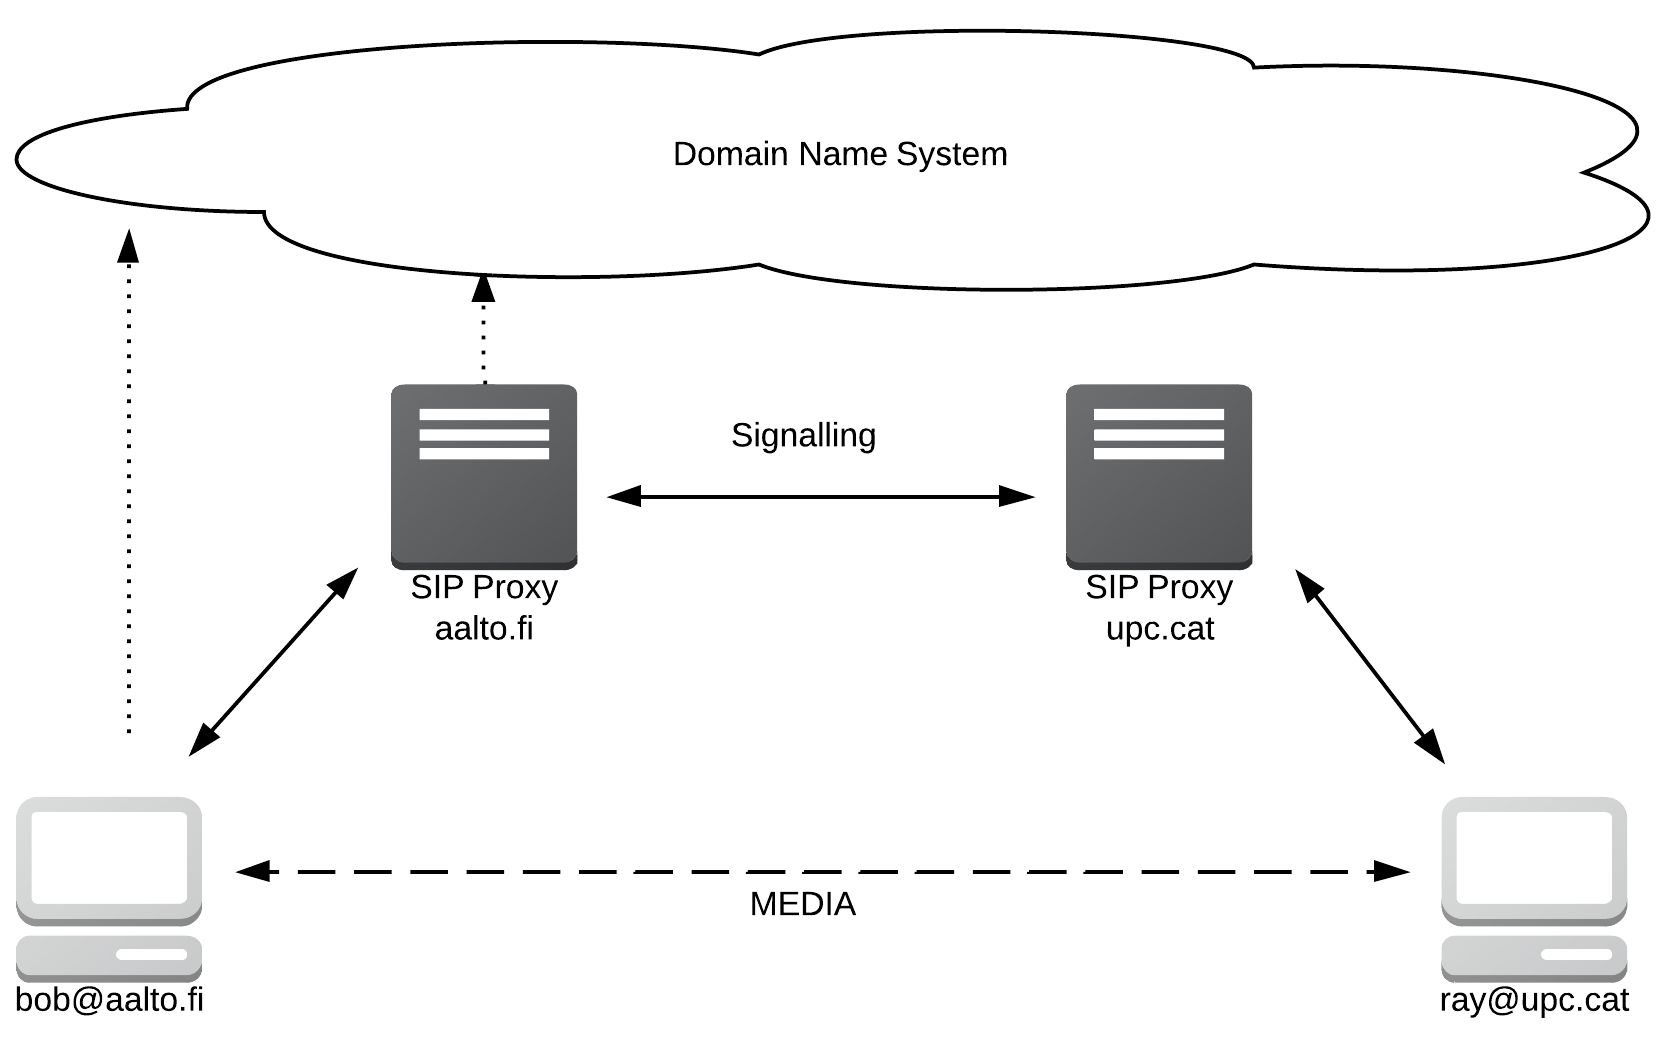
\includegraphics[width=1\textwidth]{./figures/SIParchitecture.png}
      \caption[SIP architecture for end-to-end signaling]{SIP architecture for end-to-end signaling.}
	\label{fig:SIParchitecture}
\end{figure}

SIP architecture relies in a trapezoid form where the Domain Name System (DNS) is used to locate the other peers of the system, once that peer is located and session is negotiated, media flows peer-to-peer directly to the endpoint. In order to build this system different agents are needed, SIP Proxies, SIP Redirect and SIP Registrar. SIP Proxies transmit the SDP and SIP messages from one peer to the other to establish communication (Figure~\ref{fig:SIParchitecture}). SIP Registrar are the machines that collect and save all the user information from the end points.

DNS provides the IP address for both proxy servers and allow the messages to be exchanged between both peers, when SIP is used the following messages are exchanged: INVITE, RINGING and 200OK. Those messages carry the SDP data inside in an object format, when ray@upc.cat receives the INVITE message from bob@aalto.fi builds the 200OK response carrying the SDP object that providing compatibility check between both peers and which options and codecs to use. SIP provides some more messages to update the already existing session or to close them. The media transport is done using RTP and RTCP that rely over User Datagram Protocol (UDP)~\cite{sipRFC}.

SIP is a pure Voice Over IP (VoIP) confederated technology that helped the community to learn about real-time P2P communication,we have used all the concepts and technologies embedded in SIP to build WebRTC.

\subsubsection{RTMFP and Adobe Flash}

RTMFP and Adobe Flash are proprietary technologies provided by Adobe, both services work together to provide multimedia and real-time communication between users.

Adobe Flash is a multimedia software that uses a plugin to work over the browser, it is used to build multimedia experiences for end users such as graphics, animation, games and Rich Internet Applications (RIAs). It is widely used to stream video or audio over webpages, in order to reproduce this content we need to install Adobe Flash plugin in our computer. It also carries different programming languages that drops from the standards called JavaScript Flash Language (JSFL) and ActionStript. Due to the need of using a plugin his extension to tablets and mobile devices is more complicated than using standards. Adobe Flash Player is available in most platforms except iOS devices and reaches about 98 of all internet-enabled desktop devices. This plugin allows developers to access media streams from external devices such as cameras and microphones to be used along with RTMFP.

RTMFP uses Adobe Flash to provide media and data transfer between two end points. This system usually works over UDP~\cite{rtmfpDraft}. Differing from SIP, this protocol is a full suite for media/data transfer in a P2P constraint environment and carries its own signaling methods and codecs. It also handles congestion control on the packets and NAT transversal issues. One of the biggest differences is that, similar to WebRTC, is not a full communication infrastructure and both peers must be in the same working domain to be able to communicate, is not a PSTN style of communication but a point to point messaging system. This protocol is implemented in Flash Player, Adobe Integrated Runtime (AIR) and Adobe Media Server (AMS), it is used for P2P communication between all those services~\cite{rtmfpDraft}. 

This protocol is secured and encrypted, comparing with WebRTC, this issue has been addresses clearly in RTMFP by using proprietary algorithm and different methods. The RTMFP architecture is similar to WebRTC concept, it also allows reconnection in case of connectivity issues and works by multiplexing different media streams over the same media channel when handling conferences or multiple streams. For the signaling part Adobe uses a service called Cirrus (Figure~\ref{fig:RTMFParchitecture}), this service allows architectures such as: end-to-end, many-to-many and multicast~\cite{cirrusFAQ}.
 
 \begin{figure}[h]
  \centering
    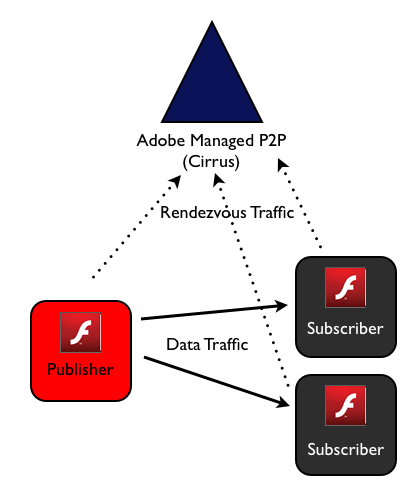
\includegraphics[scale=0.6]{./figures/cirrusAdobe.jpg}
      \caption[RTMFP architecture using Cirrus (source: Adobe)]{RTMFP architecture using Cirrus (source: Adobe).}
	\label{fig:RTMFParchitecture}
\end{figure}
 
Some of the most valuable features is the possibility to easy integrate P2P multicast topologies where one source sends a video to a group of receivers. This is something that none of the other protocols has implemented yet.

\subsection{HTML5}

WebRTC is part of the HTML5 package, both combined are an open cross-platform standard that aims to replace the Adobe proprietary proposal for P2P Real-Time Communication (RTC).

By using HTML5 features we avoid the need of installing any extra software to be able to use real-time multimedia applications on the browser.

\subsubsection{Media Capture and Streams}

HTML5 proposal will replace the existing need to use plugins when having multimedia features in web browsers. This new version carries different API that will be built into the browser and avoid the usage of external software to execute them, this scenario helps to build cross-platform standard applications in JavaScript instead of using plugins. 

Compared with the existing Adobe Flash, APIs such as Web Graphics Library (WebGL) enables developer to build HTML5 3D and 2D games that will work in any browser natively without needing any especial software but with the rendering capabilities of Flash. Mobile browsers have been more likely to adopt this new technology for rendering~\cite{webglDraft}. The first final version of the API has been already published and browsers like Chrome and Firefox carry it.

Alongside with WebGL and many other APIs, this new HTML5 also carries the new Media Capture and Streams, also known as GetUserMedia API. This JavaScript API allows developers to access local media such as video/audio from webcams and insert them in a web application by using the new video DOM element~\cite{getusermediaDraft}.

This proposal was first attached directly to the WebRTC group but has been published in a different draft, the usage of this API removes the need of using Adobe Flash to access the media device and also the plugin requirement. Developers can capture media streams from cameras and build them into Blob objects to be transmitted to other peers or reproduced locally.

 \begin{figure}[h]
  \centering
    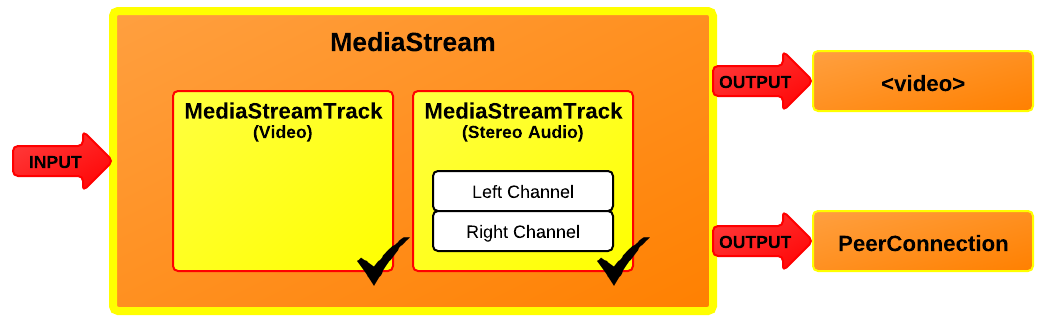
\includegraphics[scale=1]{./figures/mediastreamAPI.png}
      \caption[Media Stream API (source: W3C)]{Media Stream API (source: W3C).}
	\label{fig:mediastreamAPI}
\end{figure}

Figure~\ref{fig:mediastreamAPI} illustrates how the browser access that media and the outputs delivered to the developer. We will use this function to build WebRTC enabled applications for RTC video conferencing. The video tag is an HTML5 DOM element that reproduces local and remote streams.

\subsubsection{WebRTC}

WebRTC is a working API part of the HTML5 proposal, it is defined in a W3C draft~\cite{webrtcW3cgroup}. This API replaces the need of a RTMFP plugin for P2P communications for browsers, WebRTC uses already existing technologies, learned from SIP, bundled into an API. It is able to solve NAT transversal environments by using a mixtures of ICE, TURN and STUN technologies. For the session description it uses a modified bundled version of SDP. The format used for packet transport is RTP and SRTP, modified WebSockets are in use for P2P DataChannel implementation to provide data transport multiplexed over the same stream. All the traffic is sent over UDP or TCP over the same port~\cite{alvestrandOverview2012}.

This P2P session establishment system works in a constrained environment similar to RTMFP but it has been designed to provide legacy for other SDP based protocols such as SIP. It is a browser side API and does not provide any centralized service for signaling. Figure~\ref{fig:webrtcExample} shows how a WebRTC simple P2P scenario works, the server used for signaling is based in node.js.

 \begin{figure}[h]
  \centering
    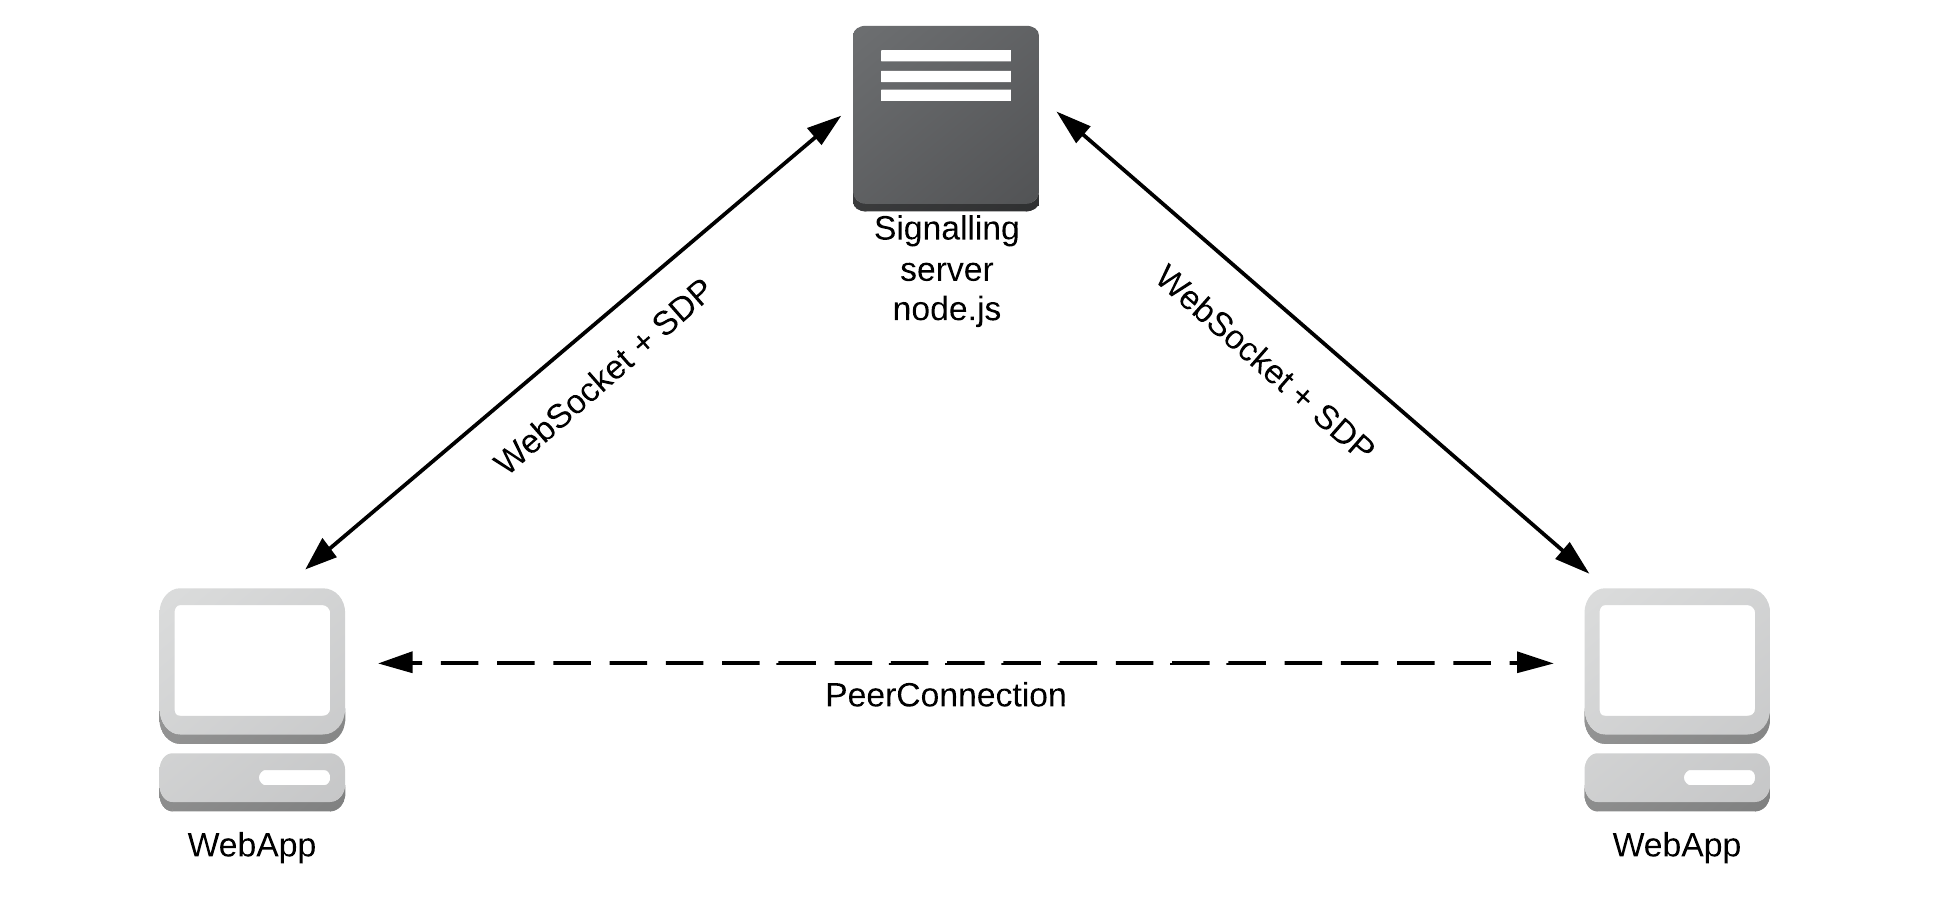
\includegraphics[width=1\textwidth]{./figures/webrtcExample.png}
      \caption[WebRTC simple topology for P2P communication]{WebRTC simple topology for P2P communication.}
	\label{fig:webrtcExample}
\end{figure}

Figure~\ref{fig:webrtcExample} does not show relay machines that provide NAT transversal solutions, those rely in other technologies that are applied to the API. In this simple example we consider both peers are in the same network without any Firewall or NAT restriction.

\subsection{Issues in WebRTC}

WebRTC uses a mixture of different technologies to perform peer-to-peer communication between clients, those technologies range from SRTP, RTP, RTCP and multiple codecs that are being discussed. This scenario makes performance the key point for success in developing stable WebRTC applications. 

Performance is manly related to computer capabilities and the ability to encode/decode at the same time as transferring and monitoring multiple peer connections. All those tasks are run over the browser and not directly on the OS, this is good for interoperability between platforms but bad in the performance aspect. Compared to Adobe technologies which uses a plugin, the performance they can deliver should be higher as they do not use as many application layers.

Media applications are delay sensitive and require a low packet loss for its proper function, WebRTC is working on this aspect by trying to implement congestion control over the connection stablished between peers, this work is not completed yet and will arise as a problem in the near future. Packet loss due to system capacity and bandwidth are measurable in WebRTC using the Stats API, this API provides information about the PeerConnection performance and is accessible by JavaScript.

Media constraints and bandwidth statistics will make a big difference in how media is acquired in WebRTC. Browsers and web applications have always tolerate some amount of delay and packet losses but this is not possible in media infrastructures for real time applications, an effort is needed to handle Quality of Service (QoS) in WebRTC to compete with RTMFP.

\subsubsection{Quality of Service}

Quality of Service (QoS) for WebRTC is being discussed and an internet draft is available with some proposals~\cite{qosWebRTCIETF}. WebRTC uses DiffServ packet marking for QoS but this is not sufficient to help prevent congestion in some environments. When using DiffServ the problem arises from the Internet Service Providers (ISPs) as they might be using their own packet marking with different DiffServ code-points, those won't be interoperability between ISPs, there is an ongoing proposal to build consistent code-points. Audio/video packets will be marked as priority using DSCP mappings with audio being more important than video or data~\cite{qosWebRTCIETF}. 

The possibility to combine QoS in the transport layer with the constraints and stats of the WebRTC API will help developers to build more adaptive applications, for example, lowing the Frames per Second (FPS) in the case of high packet losses will reduce the bandwidth usage in the case of congestion of the link. This is possible thanks to the Stats API that provide the data statistics for the peer connection.

Some environments will also require better QoS as their bandwidth will be lower, examples in the use case draft relate this to surveillance cameras or similar approaches~\cite{WebRTCcasesIETF}. In these cases QoS should be modified by using the API, this situation can lead also to malicious JavaScript injection that could flood the path with packets. 

\subsection{Security concerns}

In order to establish a call in WebRTC we use a web server for the signaling part, on the browser side we rely on built-in standardized JavaScript calling APIs which are used by the web server to establish the call between two peers~\cite{WebRTCcasesIETF}. Figure~\ref{fig:webrtcExample} represents the simple topology for a WebRTC call, even this system is similar to other provided VoIP services, the web server is able to move logic from the JavaScript in the browser giving total control to the server.

Obviously, this system poses a range of new security and privacy challenges different from traditional VoIP systems. It has to avoid malicious calling or having a call established without user knowledge, considering that those APIs are able to bypass Firewalls and NAT, Denial of Services (DoS) attacks are a threat.

Nowadays browsers continuously execute JavaScript codes from accessed web sites, this also includes malicious scripts, but in the case of WebRTC this could lead to a big privacy threat. In a WebRTC environment we consider the browser to be a trusted unit and the JavaScript provided by the server to be unknown as it can execute a variety of actions in the browser. At minimum, it must not be possible for arbitrary sites to initiate calls to arbitrary locations without user consent~\cite{rtcwebSecurityIETF}. To approach this, the user must make the decision to allow a call (and the access to its webcam media) with previous knowledge of who is requesting the access, where the media is going or both.

The previous procedure is run by the JavaScript provided by the server, this is a security issue as the user must trust an unknown authority server. Calling services commonly use HTTPS for authentication whose origin can be verified and users should be verified cryptographically (DTLS-SRTP). Browser peers should be authorized before starting the media flow, even this can be done by the PeerConnection itself by using some Identity Provider (IdP) that supports OpenID or BrowserID to demonstrate their identity~\cite{rtcwebSecurityArchIETF}. Usually this problem is not particularly important in a closed domain, cases where both peers are in the same social network and provide their profiles to the system and those are exchanged previous to the call, but it arises as a big issue when having federated calls from different domains such in Figure~\ref{fig:idpWebRTCcall}.

 \begin{figure}[h]
  \centering
    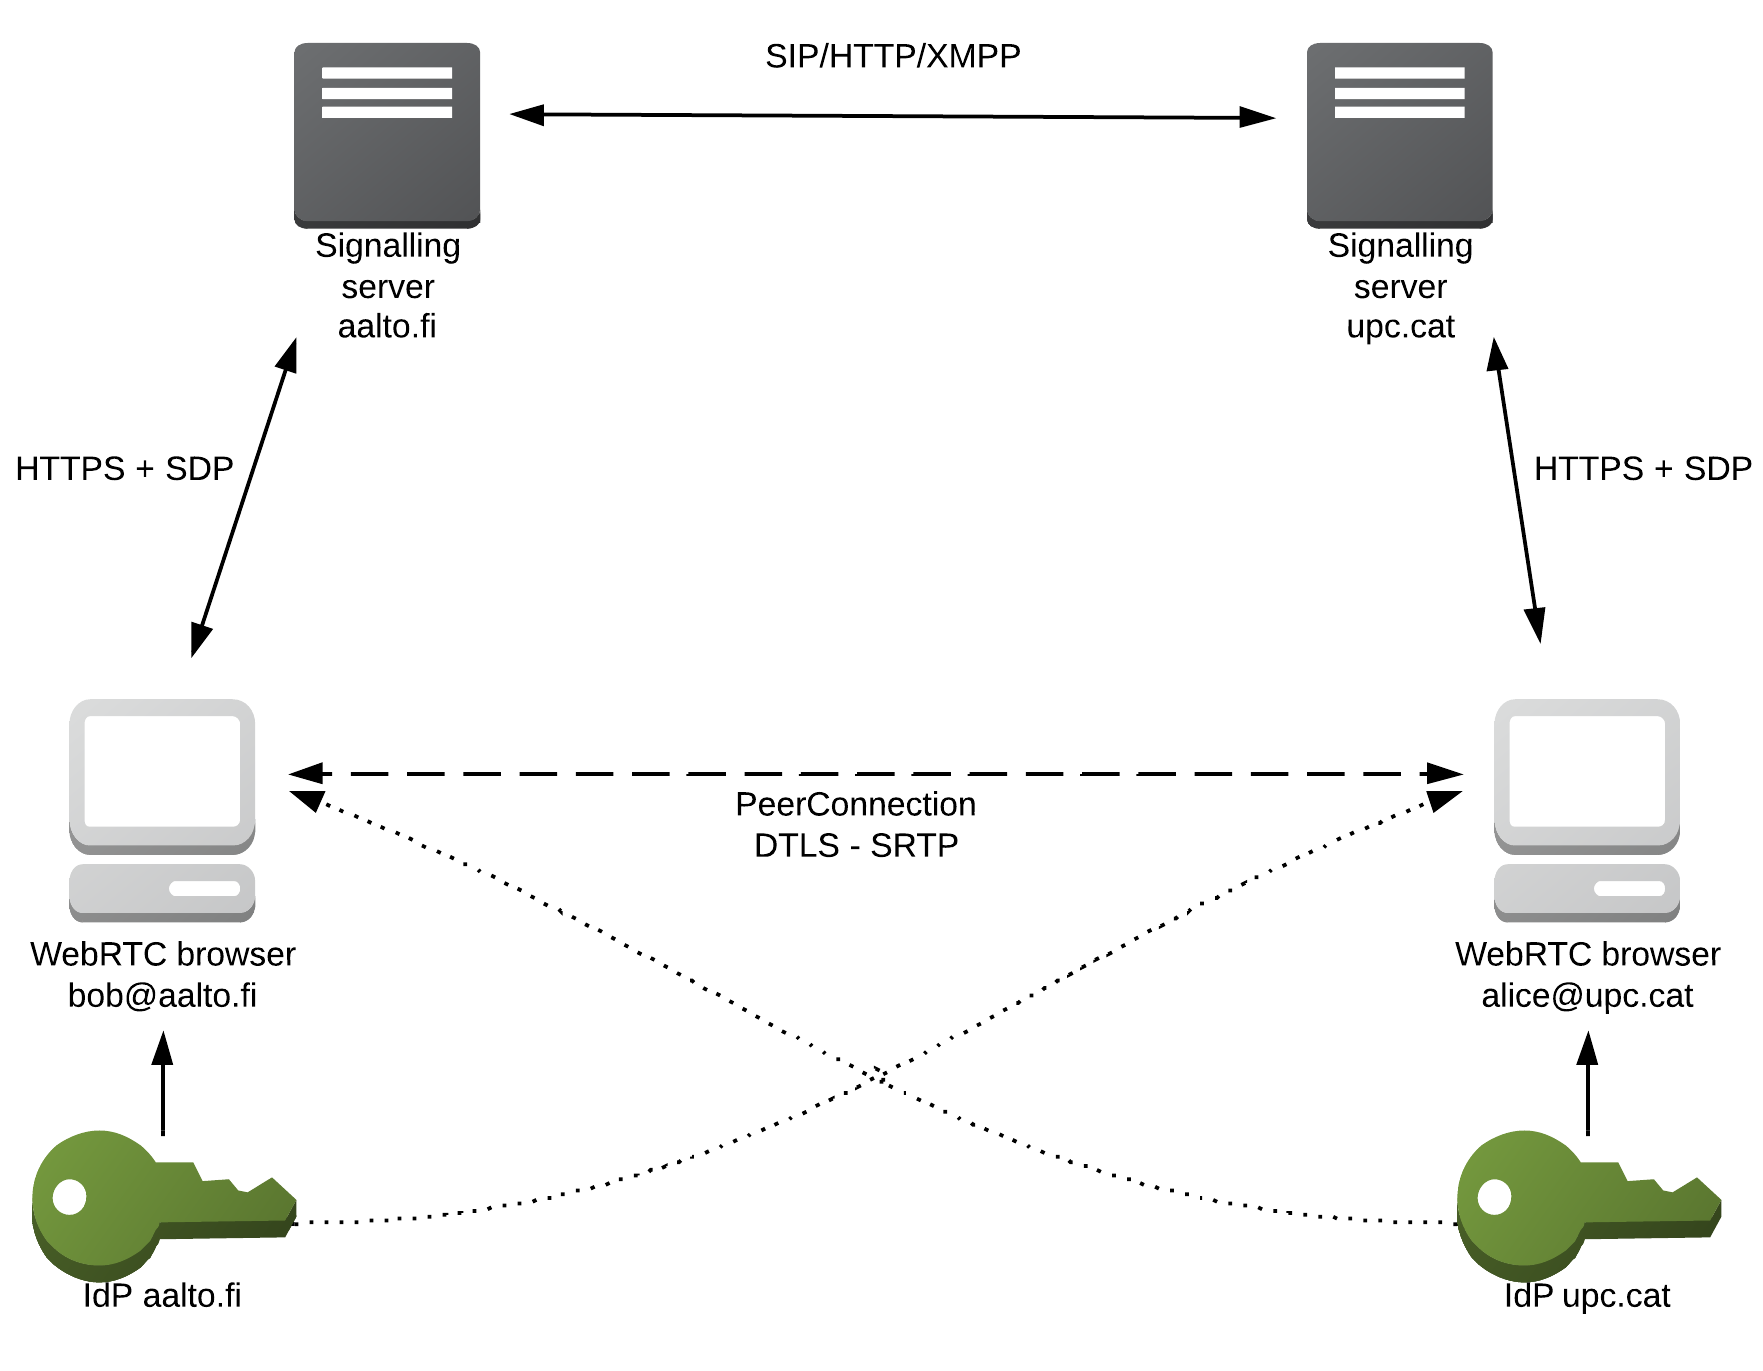
\includegraphics[width=1\textwidth]{./figures/idpWebRTCcall.png}
      \caption[WebRTC cross-domain call with Identity Provider authentication]{WebRTC cross-domain call with Identity Provider authentication.}
	\label{fig:idpWebRTCcall}
\end{figure}

If the web service is running over a trusted HTTPS certificate and has been authenticated it will be possible for the user to set the allow always access to the media, otherwise the user will have to allow this access. Once the media is acquired the actual API builds the ICE candidates for media verification. Authentication and verification in WebRTC is an ongoing discussion in the WG.

